%!TEX root = ../template.tex
%%%%%%%%%%%%%%%%%%%%%%%%%%%%%%%%%%%%%%%%%%%%%%%%%%%%%%%%%%%%%%%%%%%
%% chapter1.tex
%% NOVA thesis document file
%%
%% Chapter with introduction
%%%%%%%%%%%%%%%%%%%%%%%%%%%%%%%%%%%%%%%%%%%%%%%%%%%%%%%%%%%%%%%%%%%

\typeout{NT FILE chapter1.tex}%

\chapter{Introduction}
\label{cha:introduction}

\prependtographicspath{{Chapters/Figures/Covers/}}


\section{Biosignals and Challenges of a Data-Driven Society} 
\label{sub:motivation1}

In recent years, the continuous increase in accessible wearable technology has contributed to a significant amount of data available. The continuous production of data from wearable devices through the usage of mobile phones, smartwatches, hearables, wristbands, and other non-invasive wearable sensors has provided a valuable quantity of information. This data often comes in the form of time series, being one of the most common data types in nature \cite{puttinghuman}. As reported in \textit{Tankovska et al.}, the wearable devices usage has more than doubled in the interval between 2016 and 2019, reaching 722 million~\cite{tankovska_23_2020}, leading to a large volume of time series data being gathered in all possible scenarios, by monitoring patients in healthcare institutions \cite{cpd_medical_1, cpd_medical_2, cpd_medical_3, cpd_medical_4, dataset6, dataset7}, tracking everyday activities of humans \cite{cpd_har_1, cpd_har_2, review_1}, recording machines in industrial processes or workers motion while performing their tasks \cite{antonio, sara}. 

It has never been so easy to gather data about any aspect of our life, work, education, society, or industry. Of course, having relevant information about a subject is beneficial, but the overwhelming amount of data brings tremendous challenges in the ability to save, process, analyze and retrieve interpretable and meaningful information from which we can act upon\cite{bigdata}. Ultimately, it becomes even harder to have data well structured and labeled, considering that it is a sensitive and time consuming process, and complexity increases with data quantity. In the work of \textit{Roh et al.} is mentioned that data scientists only rely on a small portion of the available datasets because it is too expensive to label all the data available \cite{roh2019survey}, and this is just an example of how much data can be unused. This is particularly problematic when developing machine learning applications, as data should be correctly pre-processed and labeled to be sure not to include noise, artifacts or mislabeled segments of the signal (\textit{Garbage-in Garbage-out} - \textit{GIGO}) \cite{roh2019survey}.
\par
We believe that we should do more with the data we have and for that, tools should be available to support and help analysts to accelerate the process of information retrieval from time series. Both for analysts that are (not) familiar with time series data mining. Having more informative, expressive, and intuitive methods for the analysis of such data, increases the speed of analysis for experienced analysts and promotes the democratization of this analysis for less or non-experienced analysts \cite{democratize}.
\par
In this thesis, we propose novel methods that contribute to the information retrieval problem on time series. The reader will find two main domains of methods focused in (1) \textit{unveiling the grammar of time series} and (2) \textit{a language for time series data mining}. The proposed methods are designed to help in (1) explaining the \textit{story} that originated the time series through a visual representation that highlights its structure and organization and (2) making the search for patterns and events with expressive queries, moving towards human interpretable and readable time series analysis. As the reader may notice, our topics merge the concepts of time series with text. Then, the reader may appreciate that we dwell on what we believe is the \textit{linguistic nature} of time series.  

\section{Linguistic Nature of Time Series}
\label{sub:context1}

Time Series are a visual domain, from which humans can create a good intuition. It is inherent to our ability to see relevant structures and patterns. The reader can imagine a recurrent shape, such as the \textcolor{myblue}{QRS complex} of an \gls{ecg} signal that is interrupted by a \textcolor{myred}{noisy} segment (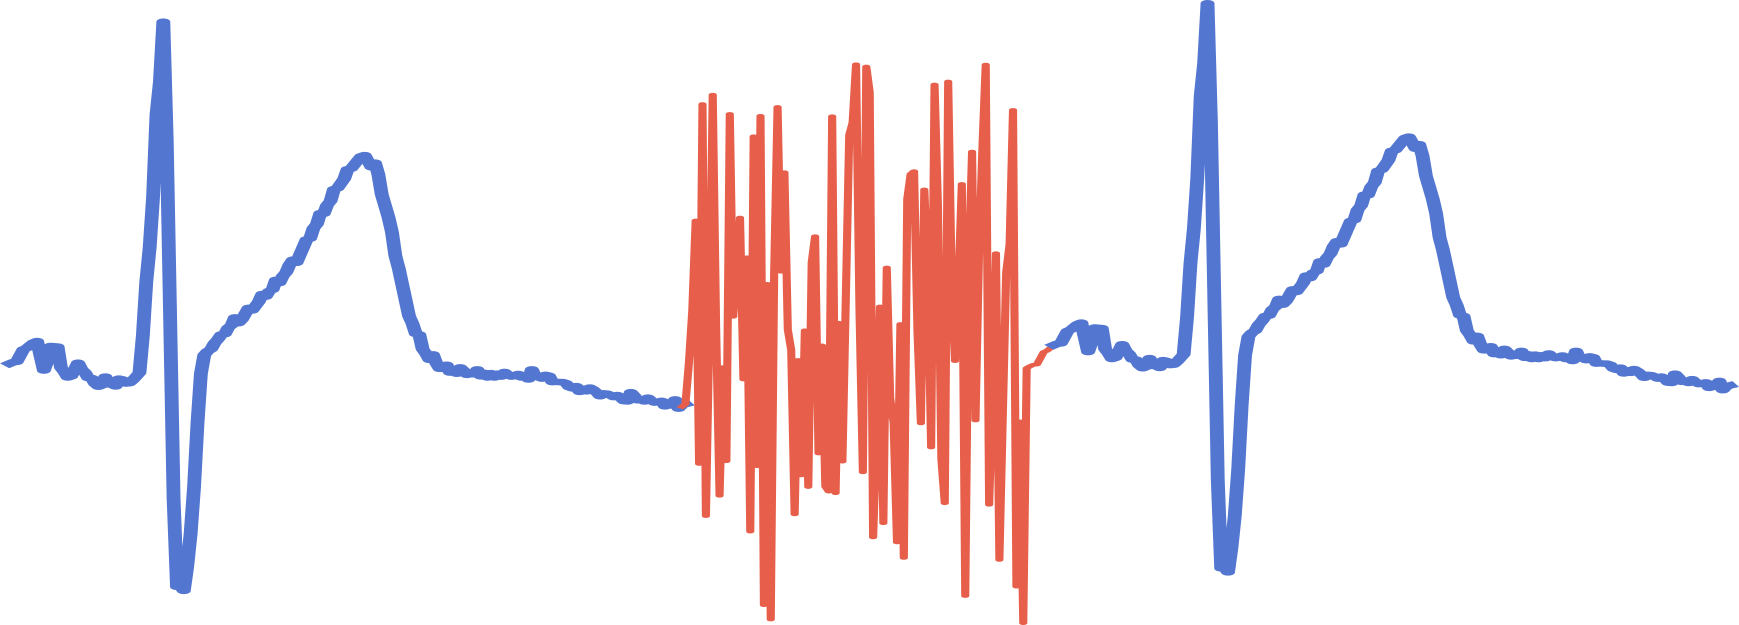
\includegraphics[height=3ex, valign=m]{ecg_noise_thumbnail.png}). When interpreting this signal, we see that it has 3 representative segments and that the first is very similar to the third one. We could then represent the signal by \textit{\textcolor{myblue}{A} \textcolor{myred}{B} \textcolor{myblue}{A}}. Some shapes may be harder to distinguish, for instance, consider an accelerometer signal of a subject while \textcolor{myblue}{walking} and shifting to \textcolor{mygreen}{jogging} regime (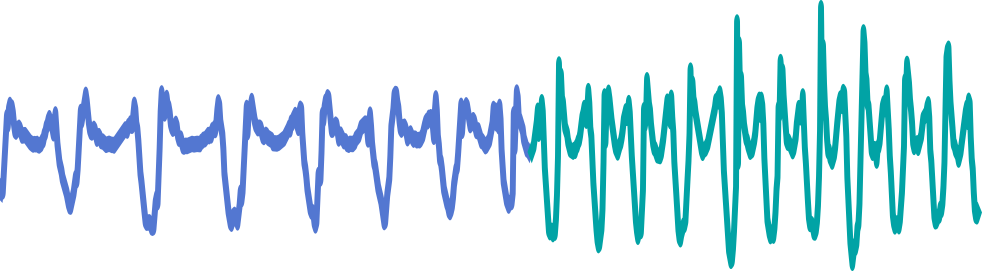
\includegraphics[height=3.5ex, valign=m]{walking_jogging.png}). Or a change in the shape of the arterial blood pressure (ABP) signal when there is a change in the subject's posture (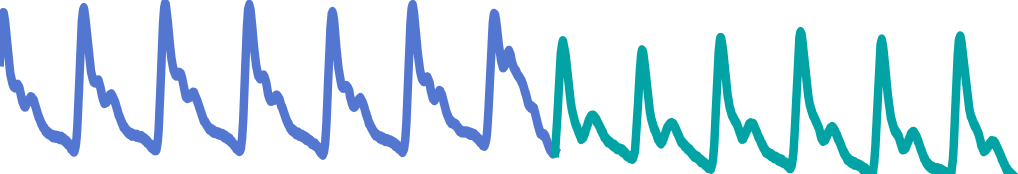
\includegraphics[height=2.5ex, valign=m]{bvpABpng.png}). In both cases, the signal has 2 structures of a similar representative periodic pattern (\textcolor{myblue}{A} \textcolor{mygreen}{B}).

This visual intuition is also very clear when a (non-)experience analyst is searching for specific shapes or patterns in time series. The reader may agree that scientists or other professionals often resort to describe the shape they are looking for. For instance, a physician may say "\textit{I am searching for the T-wave, that represents the} \texttt{large peak}" (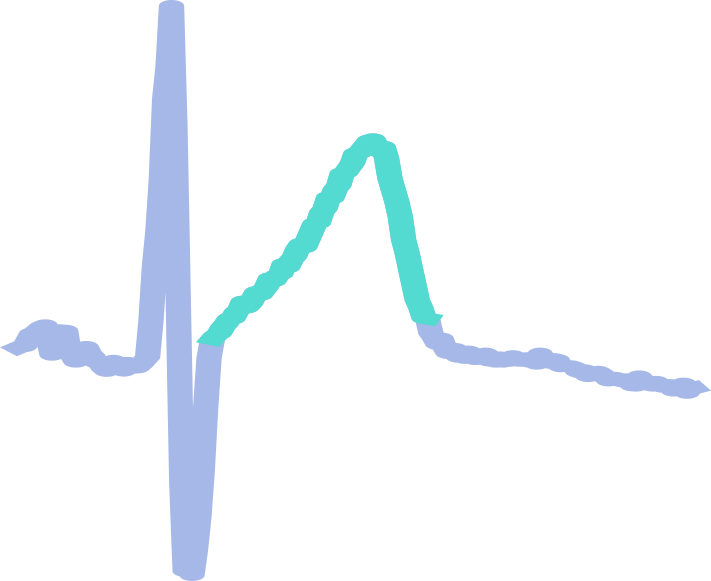
\includegraphics[height=3.5ex, valign=m]{large_peak_ecg.png}) or "\textit{I am searching for the QRS complex, that looks like a} \texttt{sharp peak followed by a sharp valley} (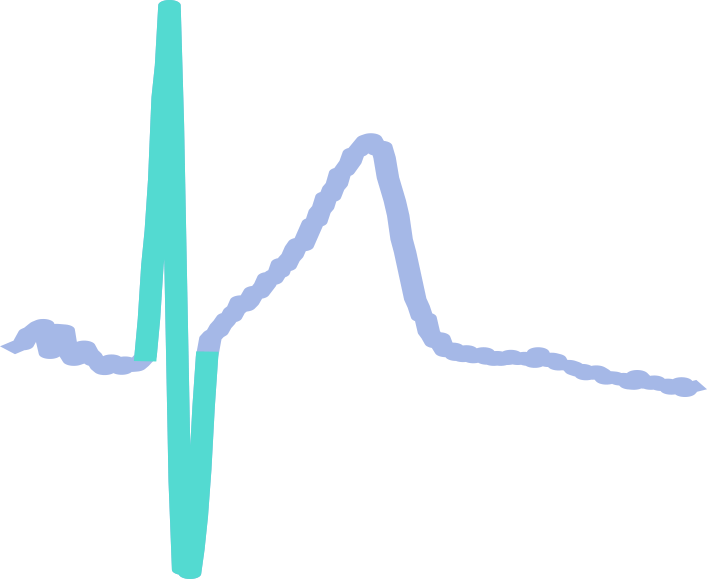
\includegraphics[height=3.5ex, valign=m]{high_peak_ecg.png})". This visual intuition also happens when analysts are trying to find differences between classes of signals. For instance, the following shapes (1) 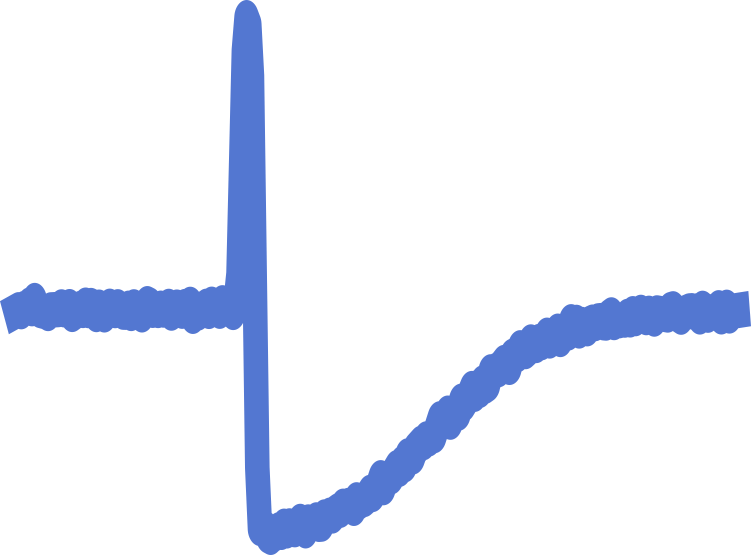
\includegraphics[height=2.5ex, width=3.5ex, valign=M]{trace1.png} and (2) 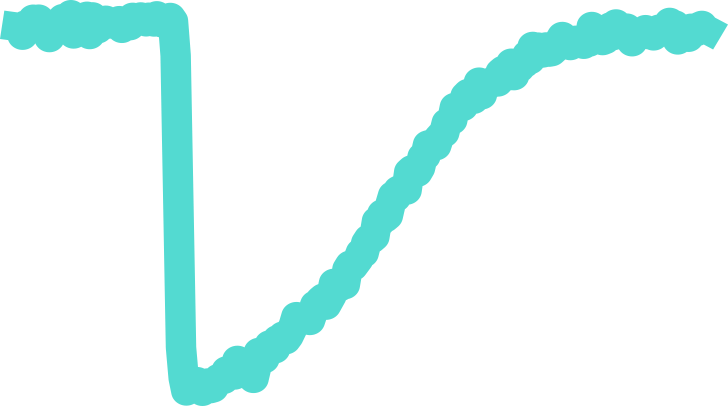
\includegraphics[height=2.5ex, width=3.5ex, valign=M]{trace_2.png} are different because "\textit{shape 1 has a} \texttt{peak} \textit{where shape 2 doesn't}". 

Time series are carriers of information and the presence of a change in the regimes of a time series or the presence of a specific shape in a segment of a time series may be associated with a specific occurrence in the physical world and be attributed to a meaning. This notion of structure and meaning is a good approximation of what represents the foundation of a language: grammar and meaning~\cite{grammar}.

\textit{Grammar} is generally defined as the book of rules that constitutes the structure of a language and is modeled by the morphology and syntax \cite{grammar}. The first is the structure of words, how these are built or morphed based on context, while the latter consists in organizing words in sequences to form larger linguistic units, such as sentences. Just as a language has morphological and syntax rules that represent its structural information, time series are also organized by a formal structure of ordered subsegments with specific morphological characteristics, organized to build larger segments. Our first topic is related to \textit{unveilling} this structure with methods that can parse it.
\par
In addition to a \textit{grammar}, a language also has \textit{meaning}. The \textit{meaning} on time series depends on the context and what occurred in the physical world that is seen on the signal. Specific occurrences might be attributed a specific meaning by an analyst, as we have seen above with the physician example. In this work, we explore a language to \textit{translate} time series into text and use this textual information as an expressive way of searching for meaningful events and patterns. This is related to our second topic, which focuses on using language in time series data mining tasks.
\par
Until now, we have been using the term \textit{time series}, but the thesis is entitled \textit{A Language for Biosignals}. Having explained how time series have a \textit{linguistic nature}, we now focus our attention to a specific domain of time series, \textit{biosignals}, which are time series that come \textit{from} the \textit{human body}, such as the \textit{heart} (\gls{ecg} - ), \textit{muscles} (\gls{emg} - ), \textit{brain} (\gls{eeg} - ) or even movements (\gls{imu} - ). Considering that the tools developed can be employed in any time series domain, we will use this term instead, but we will give most of our examples from occupational \textit{biosignals}, with a special interest in showing how these can be helpful and meaningful in the context of occupational health.

\section{Biosignals: Context and Relevance in Occupational Health} 
\label{sub:context2}

This thesis was developed in a strong partnership with the \textit{Ergonomy} team from \textit{Volkswagen Autoeuropa}. Therefore, the central domain of the application regarded the analysis of \textit{biosignals} from workers to retrieve meaningful information about their occupational risk status and prevent \gls{wmsd}s. \gls{wmsd}s prevail as the most common occupational disease in the European Union. These have a global impact on the well-being of individuals and their quality of life in a range of working sectors \cite{Irastorza2010}, accounting for the second-largest responsibility to disability worldwide \cite{Luttmann2003}. These are especially prevalent as upper limb or neck disorder (with 42\% of all \gls{wmsd} cases reported) \cite{Seidel2019} in several industry sectors, such as textile and automotive, where production processes with pre-defined motions and actions have a repetitive/cyclic nature. This has a negative impact on the risk to develop musculoskeletal disorders, with tremendous consequences to both workers and companies, leading to absenteeism, early retirement, and loss of productivity \cite{Trabalhadores, Varandas19}. 

Several strategies have been implemented to identify, regulate and prevent occupational risks in manufacturing industries, such as (1) the inclusion of job rotation schedules, which promote a variation of the exposure throughout the working day \cite{jobrotation1, jobrotation2} and (2) screening tools, for the assessment of occupational risk exposure, e.g. \gls{ocra}, \gls{rula} or the \gls{eaws} \cite{ocra, rula, eaws}. Nevertheless, these strategies are not optimal because they (1) are not automated, relying on observational methods and dedicated personnel to inspect video records; (2) are not objective measures; (3) do not take into account differences among the worker's population, as anthropometric, age and experience variability; and (4) present single scores, being insufficient to explain the factors that contributed to this risk. With the advent of Industry 4.0, more companies are using modern strategies that follow digital solutions to provide direct and objective quantitative measures \cite{romero}. An example of these incentives is the usage of \textit{biosignals}, with wearable inertial devices for physiological, motion, and posture tracking of workers.

From \gls{imu}, time series can be collected and relevant information can be directly measured, e.g. position and velocity of each body segment, postural angles between joints, and gait parameters, making these important for ergonomics studies \cite{Caputo2019, Hang19}. There are some limitations to using \gls{imu}, mostly related to the long-term bias (sensor drifting) arising from long acquisitions and the empirical process to fine-tune sensor fusion techniques. Other systems can be used for motion capture, such as camera-based methods, but these rely on a fixed setup of cameras, which is unmanageable in real industrial scenarios \cite{sara}. In addition to motion sensors, the inclusion of physiological sensors, such as \gls{ecg}, \gls{emg} and even \gls{fnirs} can give reliable evidence of other occupational health variables, namely cardiovascular load, muscular activation, cognitive effort and fatigue \cite{silva_rip, cardiovascular_load, rythm_cyclic_work, rui_varandas}.

The usage of biosignals in this context can play an important role in supporting the decision of ergonomists and other professionals in the industry. To develop systems that can use physiological, motion, and postural data for direct risk assessment and reporting, several challenges arise in the time series data mining domain. For instance, considering the periodic nature of most manufacturing tasks, risk factors are calculated by working cycle. Therefore, methods should be developed to identify working cycles with some variability in their periodicity. In addition, real occupational scenarios might have interruptions or changes in the working behavior, due to abrupt production stoppage, shift breaks, or even because the worker shifted to another workspace that has a different movement pattern. 

Other questions also arise by ergonomists, such as \textit{can we find a pattern that has a sharp rise in the \gls{imu} from the arm?} or \textit{when the worker is using a hand tool to rotate a screw, can we see a periodic pattern on the \gls{imu} from the hand?}, which represent specific patterns with a descriptive shape that can be seen on the signals and are specific of a task. These events can be relevant to studying their precise impact on the worker's occupational exposure. Having ways to detect these patterns is of great relevance as well. In this study, we will show how the proposed solutions can have an impact on these problems, and how they contribute to providing relevant visual feedback for information retrieval from the occupational data and make the search for specific patterns more intuitive and expressive, even for non-experienced data analysts, such as ergonomists.

%This would also help counteract the lack of usability of data by moving towards a \textit{democratized} usage of time series by non-experienced scientists \cite{democratize}.

\section{Research Paths}

The previous sections introduced the topics explored in this thesis for information retrieval on time series, our main motivations to develop the proposed methods, and how these can have significant contributions in the biosignals domain, more specifically for occupational health data.
\par
The work in this thesis contributed to all layers related to time series, from the moment data is acquired (\textit{sensing}), processed for information retrieval (\textit{analysis}), and how it is used to act upon (\textit{decision making}). From these, the presented work in this document will especially address the development of methods for information retrieval (\textit{analysis}) from time series for better \textit{decision making}.

\begin{enumerate}

\item \textbf{Sensing} - Explore in depth the available technology to measure motion and postural variables in occupational scenarios for risk assessment. This will take into account which variables are associated with a risk, based on ergonomic standards. These measures are returned as time series, which are processed in the topic \textit{analyzis};

\item \textbf{Analysis} - In this topic, three main research paths are explored with specific research topics. \textbf{A -} (1) study how to perform structural information retrieval in time series for segmentation based on change points and periodic points and (2) how are the segments related based on their similarity. For this, we applied a feature-based transformation of the time series and similarity-based measures to make a meaningful visual representation, from which the segmentation points can be extracted and the relationship between segments can be made. \textbf{B -} explore a symbolic representation of time series and a word feature-based representation of time series, studying how these can be used for more expressive and intuitive pattern search with the help of regular expressions and ultimately natural language. \textbf{C -} From the textual representation of time series, study if we can make a higher leveled distance measure, following standard text mining methods. The resulting outputs of these methods can ultimately be used to be more aware of why a signal is different from the others.

\item \textbf{Decision Making -} Discuss how the developed methods can contribute to more aware and informed decisions. Considering the outputs of the methods developed in research path A, how can the analyst gain intuition over the structure of the data associating it with what happened in the physical world. In what regards to research path B, how expressive is the process of searching for specific events and patterns with the proposed linguistic-based search methods.

\end{enumerate}

\section{Thesis Structure}
\label{sec:structure}

\begin{figure}
\centering
\includegraphics[width=\linewidth]{intro_thesisstructure.pdf}
\caption{General topics contemplated on this thesis and structure of the document. It highlights the 3 layers of involvement related to time series: Sensing, Analysis, and Decision Making, focusing on the Analysis layer, which includes two major topics subdivided into 4 sections each.}
\label{fig:intro}
\end{figure}

This thesis provides a detailed description and explanation of the research work developed during the Ph.D. program. It is organized into nine Chapters, each contributing to telling the story of this thesis. The reader may appreciate Figure \ref{fig:intro}, which illustrates a guideline of the structure of this work, with a short description of each Chapter's topics and content. \textbf{Chapter 1} introduced the main motivations, goals, and context for the development of the proposed methods. \textbf{Chapter 2} provides the reader with the fundamental definitions and knowledge needed to have a clear picture of what is developed in this work.\textbf{Chapter 3} depicts the state-of-the-art works related to what we developed, namely in the topics of segmentation, summarization, pattern/event search and classification.\textbf{Chapter 4} describes the data we used, explaining its source for both private data and publicly available data, for which purposes it was used and how it was used in this work.\textbf{Chapter 5} explains the algorithm developed for time series structural information retrieval (Unveiling the \textit{Grammar} of Time Series) and provides examples of its usage for novelty segmentation, periodic segmentation, similarity profiles, and query search. \textit{Chapter 6} covers the usage of language for time series data mining (A \textit{Language} for time series data mining), more specifically introducing a novel symbolic approximation and how it can be used for pattern search and classification. In addition, it also explains how to use natural language with a word-feature-based representation of time series. \textbf{Chapter 7} shows the application of the previous methods to an exhaustive set of examples, namely from the occupational scenario, and presents major results. In addition, this chapter also provides a general discussion of these and how the proposed methods can be used for the benefit of the analyst. \textbf{Chapter 8} gives an overall remark on the outcomes of this thesis and a reflection on the contributions that the developed methods have in making time series preparation and data mining more expressive, quicker, and more practical for an ever-increasing number of data available. It also provides the reader with a clear idea of which are the future paths for this work in terms of novel applications and performance improvement.

%Chapter 2 introduces theoretical concepts necessary to have a complete understanding of the work developed. It covers an introduction to motion and postural sensors used in occupational settings, time series, standard methods for its representation and analysis, and text mining concepts. 